%!TEX root = paper.tex
%%%%%%%%%%%%%%%%%%%%%%%%%%%%%%%%%%%%%%%%%%%%%%%%%%%%%%%%%%%%%%%%%%%%%%%%%%%%%%%%
\section{Fundamental Game Properties}
\label{sec:gamemechanics}

This section will focus on describing the main game loop and the 
framerate and both their implications for properly measuring video 
games. On a technical level these two properties distinguish passively 
consumed videos and video games the most.


%%%%%%%%%%%%%%%%%%%%%%%%%%%%%%%%%%%%%%%%%%%%%%%%%%%%%%%%%%%%%%%%%%%%%%%%%%%%%%%%
\subsection{The Framerate}
\label{sec:framerate}

In contrast to traditional video media with their fixed framerates of, 
e.g., \SI{24}{\hertz} or \SI{29.97}{\hertz}, video games are more 
flexible but simultaneously also much more demanding to the framerate. 
Generally speaking, motion in video data is based on the principle of 
\textit{apparent motion}. In order to perceive objects to be in motion 
in videos, consecutive images have to appear at a certain rate which is 
considered to be at about \SI{16.67}{\hertz} according to 
\cite{wertheimer1912experimentelle}. Below that threshold objects will 
appear as two distinct objects between two consecutive frames.
%This form of apparent movement is called the phi phenomenon.
The higher the rate of displaying images, the more fluid the motion 
looks, as the discrete ``jumps'' in the position of the object get 
smaller the higher the framerate is.\footnote{One can verify this 
behavior for example at \url{https://frames-per-second.appspot.com/}.}.

In general, there is no commonly established upper limit to the 
framerate that humans can still perceive as an improvement to motion 
presentation, the gain has however diminishing returns. The typical 
movie framerate of \SI{24}{\hertz} is considered to be at the lower end 
of motion perception but mostly still works without any problem due to 
the presence of motion blur. This artifact is always present in 
recorded images as objects are still in motion during film exposure.
%A faster shutter speed reduces the amount of motion blur.
% film grain also has an influence

% \begin{figure}[!t]
% 	\centering
% 	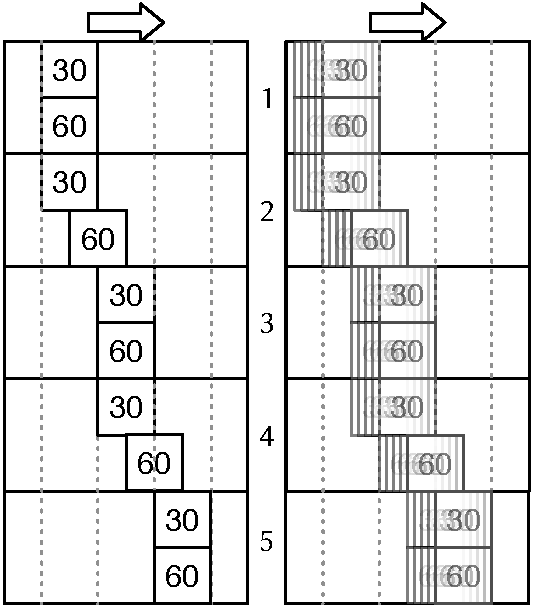
\includegraphics[width=1.0\columnwidth]{images/framerate.pdf}
% 	\caption{Effects of frame rate and motion blur on the smoothness of 
%movement and spatial resolution. Objects move at the same speed to the 
%right only the position os updated at different rates. A depiction of 
%strong motion blur was added to the right-hand side.}
% \label{fig:framerate}
% \end{figure}

The benefit of motion blur lies in its ability to conceal stutters in 
apparent movement due to the object and its edges being blurred, 
thereby reducing the positional information available on it.
%, Figure~\ref{fig:framerate} illustrates this. 
Therefore, typical movie sequences usually appear to be perfectly 
fluid. Only for example when the camera pans at a high speed stutters 
in object movement or the viewport updates become apparent. Intrinsic 
motion blur is absent in computer generated imagery but can be 
artificially added to the images. While adding blur to video games can 
improve fluidity, it also reduces the spatial information available to 
the player and hampers the precision of the player's actions. Therefore 
it is often avoided, especially for objects in focus.

Video games add two more factors to the frame rate consideration. The 
first is the issue of the monitor's refresh rate. Monitors work with a 
fixed, configurable image refresh rate, typically always including 
\SI{60}{\hertz}. If the game outputs images at an inconsistent rate or 
a rate lower than the monitor's refresh rate or if the framerate is not 
an integer multiple of the refresh rate or vice versa one of two things 
will happen:
%(depending on the implementation and the presence of vsync)

\begin{itemize}
	\item If the monitor fetches a frame from the graphics card's buffer 
while the frame is still being rendered, the result will be a mixture 
of the new frame in the upper half of the image and a frame which is 
one time interval older. This artifact is called \textbf{tearing} and 
should be avoided.
	% only the upper portion of the frame  finished, One frame split up 
%between two refresh cycles
	\item Games can also be configured to postpone the rendering of a new 
frame until the monitor has already fetched and displayed the current 
frame, this is called waiting for vertical synchronization or 
\textbf{VSYNC}. No tearing will occur, but the \gls{IAT} of new frames 
might become very irregular, displaying some frames more often than 
others just to match the monitors refresh rate, resulting in a 
stuttering display. This latter stuttering effect also occurs for 
\SI{24}{\hertz} movies being displayed on a \SI{60}{\hertz} TV screen. 
Therefore most TVs additionally provide a dedicated \SI{24}{\hertz} 
refresh rate mode to remove the stuttering.
\end{itemize}

Finally, video games also distinguish themselves from video material by 
being highly interactive. Specifically this means that video games 
constantly require inputs on short time scales to which the game reacts 
and displays the feedback. Therefore, the framerate also influences the 
reactivity of a game and can be a source of latency as discussed 
further in Section~\ref{sec:latency}.


%%%%%%%%%%%%%%%%%%%%%%%%%%%%%%%%%%%%%%%%%%%%%%%%%%%%%%%%%%%%%%%%%%%%%%%%%%%%%%%%
\subsection{Game Tick Rates and Send Rates}

At their core video games are essentially feedback-directed real-time 
simulators. The simulator's main loop consists of three central parts 
as depicted in Fig.~\ref{alg:gameloop1}. Every render-call means 
putting out a new video frame. As this framerate is usually not limited 
and variable, the game logic has to update its state on a time-scale 
operating independent of the current frame. Some games also update 
parts of the game on a fixed frequency, the so-called 
\textbf{tickrate}, for example a non-game-influencing physics effect 
updating at a lower \SI{30}{\hertz} rate.

%Some games do not do this and tie the game time directly to the frame 
%rate and expect to be run at a fixed frequency. If one manages to 
%unlock the frame rate in such games, the game will often run much 
%faster with numerous mostly disadvantageous side effects. Examples 
%include games optimized for older CPUs and clock speeds now 
%unexpectedly running at much higher clocks. Also games such as Need for 
%Speed Rivals, which was locked at 30 fps, but could be unlocked and 
%subsequently behave erroneously. Also, games with a locked frame rate 
%are very much frowned upon in the gaming community, especially when the 
%cap is lower than 60 fps.
%This general logic is also preserved in modern multi-threaded game 
%designs, although it is more difficult to achieve.

\begin{figure}[!t]
\centering
\removelatexerror
\begin{algorithm}[H]
 \While{game running}{
  read inputs\;
  update game state\;
  render screen\;
 }
\end{algorithm}
\caption{Basic model of a continuous main video game loop.}
\label{alg:gameloop1}
\end{figure}

Online video games complicate this update logic a bit. In online games, 
the client is not the final authority over its game state any more. 
Instead, interpreted input commands are sent to the server and a 
preliminary game state is calculated locally. When the authoritative 
update from the server is received the two states can be once again be 
synchronized. A typical scenario with all the relevant rates for an 
online game running in a cloud gaming environment is depicted in 
Fig.~\ref{fig:tickrate-streamed}. To make matters even more complicated 
the rates of sending input commands from the clients to the server as 
well as game state updates from the server to the clients do not need 
to be the same rate as the server's tick rate. Popular examples for the 
fixed tickrates of game servers include \SI{64}{\hertz} or 
\SI{128}{\hertz} for \textsc{Counter-Strike: Global Offensive}, 
\SI{20}{\hertz} for \textsc{Minecraft}, or \SI{30}{\hertz} for 
\textsc{Dota 2}.

\begin{figure}[!t]
	\centering
	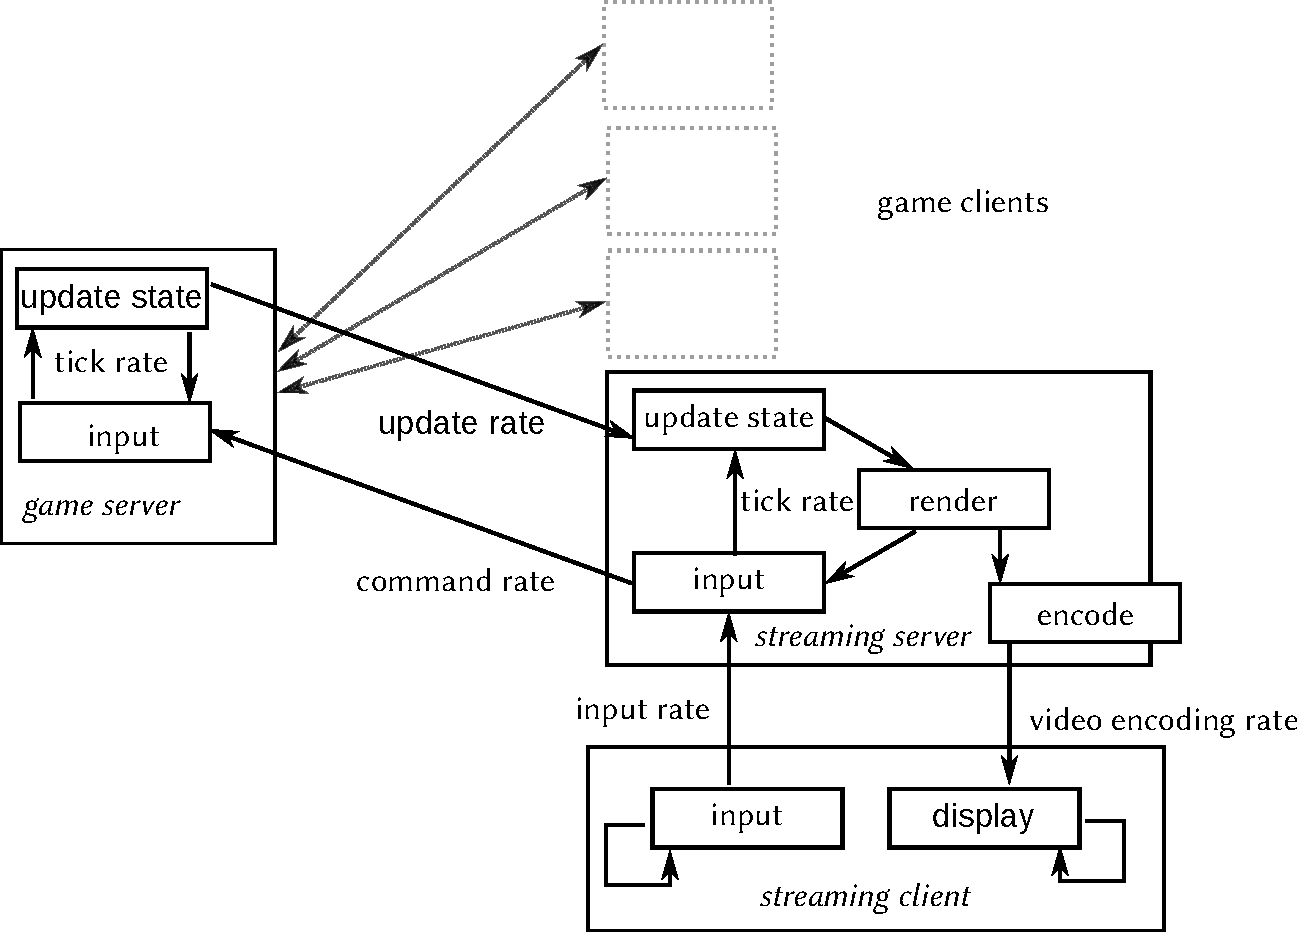
\includegraphics[width=1.0\columnwidth]{images/game-tick-rate-streamed.pdf}
	\caption{Interaction of client and server in streamed online games.}
\label{fig:tickrate-streamed}
\end{figure}


%%%%%%%%%%%%%%%%%%%%%%%%%%%%%%%%%%%%%%%%%%%%%%%%%%%%%%%%%%%%%%%%%%%%%%%%%%%%%%%%
\subsection{Sources of Latency in Gaming}
\label{sec:latency}

It is evident that latency is a critically important factor for online 
games, for fast games, or especially for competitive games as will be 
discussed in Sec.~\ref{sec:game-criteria}. But besides the obvious 
network delay there are many more sources of delay that need to be 
factored in when examining these games, including the input device, the 
time to sample and process the input, the game engine and server and 
their tickrates, frame rendering time, and ultimately the time to 
display the frame on the monitor. Only if all sources are factored in 
the complete \textbf{end-to-end lag} is captured. What makes matters 
even worse, is that this lag is usually not constant but can vary 
depending on the type of action triggered by the input. While some 
simple actions, say opening the menu, may have a very short lag, more 
complex interactions, e.g., issuing a move command, may take 
considerable longer to complete especially when the game is not 
performing well, partly due to the actions taking more than one game 
tick to complete. Therefore, each video game will have a distinct ``lag 
profile''.  Fig.~\ref{fig:tickrate-timeseries} shows a time series 
attempting to exemplify this for the simplified case of an online video 
game.


\begin{figure}[!t]
	\centering
	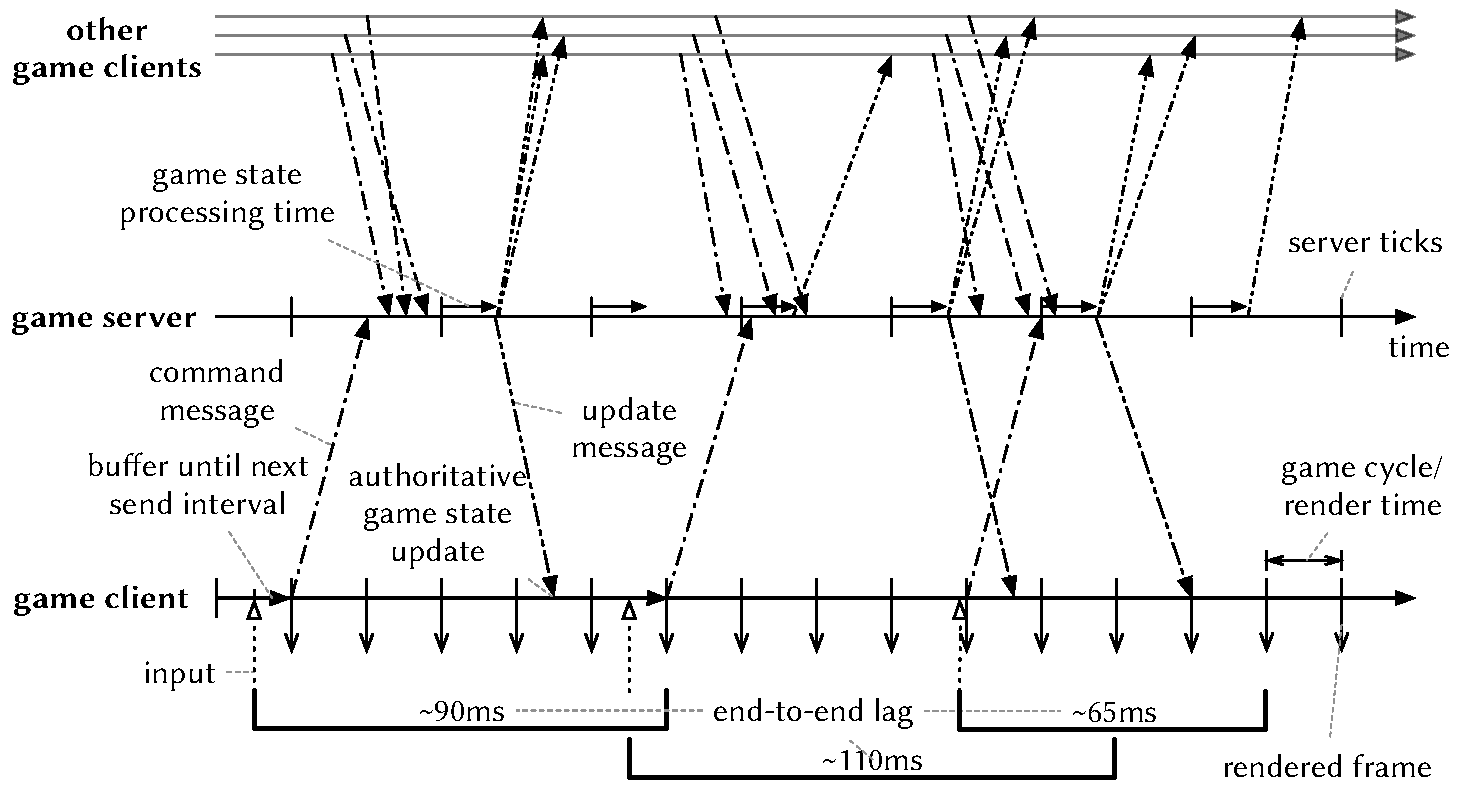
\includegraphics[width=1.0\columnwidth]{images/tickrate-timeseries.pdf}
	\caption{Exemplary time series of an online video game's client-server 
interaction and resulting end-to-end lag. Delay values are given for a 
framerate of \SI{60}{\hertz} and a server tickrate of \SI{30}{\hertz}, 
the network latency will only show minor variations.}
\label{fig:tickrate-timeseries}
\end{figure}

To demonstrate the effects of all the involved parameters, a 
MATLAB-based queuing simulation closely resembling the interactions 
given in Fig.~\ref{fig:tickrate-timeseries} was set up. With this the 
influence of any of the lag sources can be easily simulated and the 
biggest culprits identified. For example, the influence of the 
framerate on online games becomes evident in 
Fig.~\ref{fig:e2e-delay-sim}, where increasing the framerate from 
\SI{15}{\hertz} up to \SI{120}{\hertz} can significantly reduce the 
game's lag, a result that can also be easily applied to cloud games, 
where streaming often operates at a lower framerate to conserve 
bandwidth.

%All in all, if possible, video game measurements should always 
%consider the full \textbf{end-to-end} lag factoring in every possible 
%source of delay but also the presence latency compensation and 
%concealment techniques.


\begin{figure}[!t]
	\centering
	%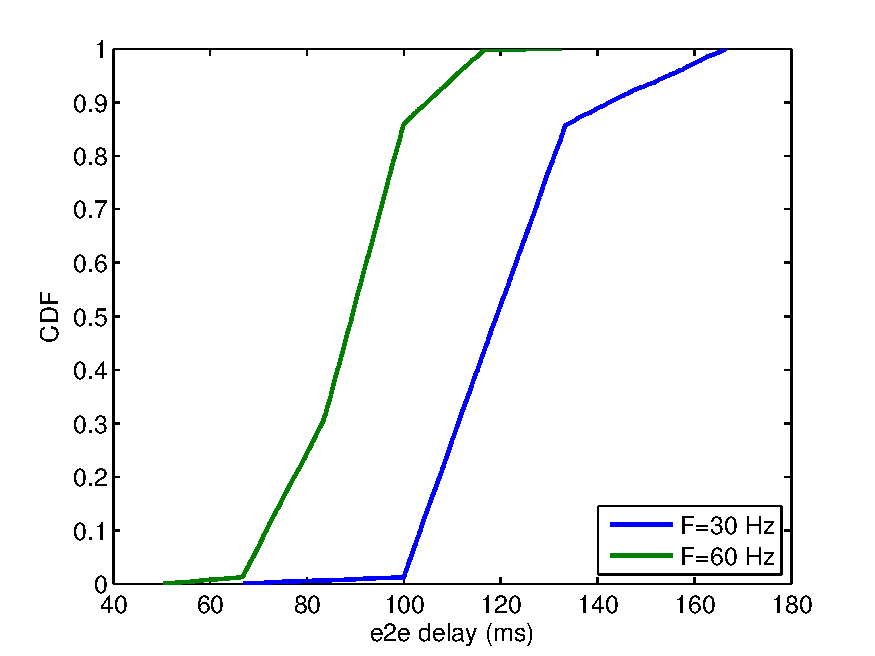
\includegraphics[width=1.0\columnwidth]{images/e2e-delay-sim.pdf}
	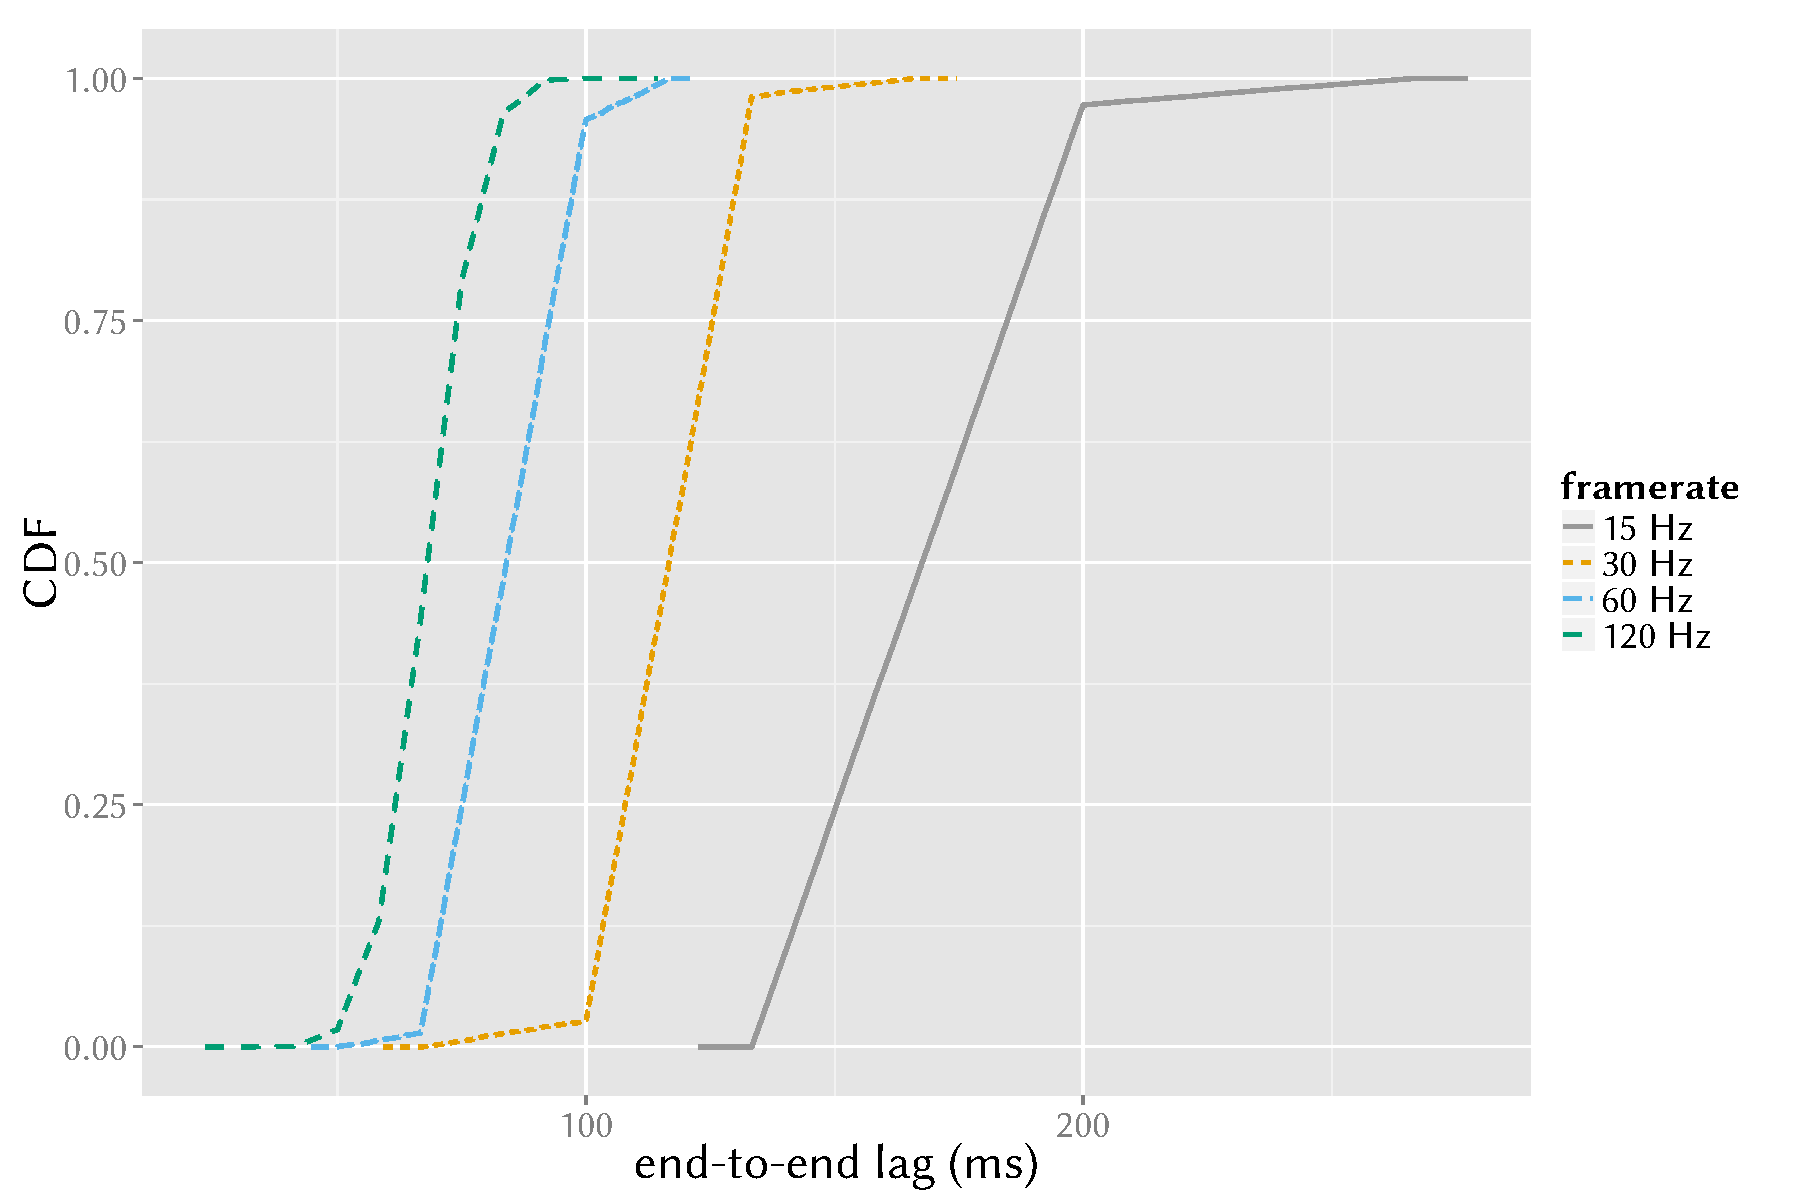
\includegraphics[width=1.0\columnwidth]{images/R-gamesim.pdf}
	\caption{\acrshort{ECDF} of a simulated online video game interaction 
and the resulting end-to-end lag depending on the game's frame rate. 
One-way network delay followed a Gaussian distribution with $\mu = 
\SI{20}{\milli\second}$ and $\sigma = \SI{5}{\milli\second}$. The 
server's tickrate was set to \SI{60}{\hertz}.}
\label{fig:e2e-delay-sim}
\end{figure}




% Online games attempt to compensate network latency through various 
%means, such as already showing the results of your local inputs while 
%waiting for the authoritative update from the server and potentially 
%rolling back the local updates.

% TODO: Also mention lag compensation/concealment techniques:
% Client-side: non-authoritatively update game state based on own 
%inputs and merging it afterwards with the server's view, correcting any 
%prediction errors
% Server-side: Keep a short history of past game states, and do not 
%execute player commands at the state they were received but rather at 
%the (estimated) state time they were intended for.

% lag compensation can also be implemtented specifically for cloud 
%gaming as the work conducted in \cite{Lee:2015:OUS:2742647.2742656} 
%suggests, however incurring siginficant overhead in terms of processing 
%time for the game logic and renderer as well as the encoding and 
%bandwidth due to specutatively generating and transmitting frames ahead 
%of their corresponding input.


% game keeps history of recent game state snapshots to interpolate 
%between two server states and create a smoother experience (thus 
%decoupling client frame rate from the server's state updates), but adds 
%e.g. \SI{100}{\milli\second} of view lag due to snapshot history.


%%
%\subsubsection{Online Video Game Latency Concealment Techniques}


% input: absolute (eg mouse) vs. relative (analog stick)
% frame perfect input
% double/triple buffering
% inputs per minute vs timing precision of input
% range of interactivity
% latency sensitivity/responsiveness of different game mechanics / UI 
%elements in the same game
% latency of camera movement / UI vs actual game elements


%Info on source engine networking: 
%\url{https://developer.valvesoftware.com/wiki/Source_Multiplayer_Networking}
%\url{https://developer.valvesoftware.com/wiki/Latency_Compensating_Methods_in_Client/Server_In-game_Protocol_Design_and_Optimization}
%(Latency Compensating Methods in Client/Server In-game Protocol Design 
%and Optimization, Yahn W. Bernier (yahn@valvesoftware.com), 2001, 
%Software Development Engineer, Valve Software)



% Online games generally follow one of two designs. Either there is a 
%dedicated server available to host the game, or one of the clients is 
%elected to additionally act as the server.
% The election is typically based on criteria such as the available 
%performance and latency. If the selected host drops out of the game, a 
%new server has to be elected and the game gets migrated there, usually 
%stopping the game for a few moments. Competitive games almost always 
%choose the dedicated approach to ensure fairness, stability and better 
%control cheats.



% \begin{figure*}[!t]
% 	\centering
% 	\begin{subfigure}[b]{0.5\textwidth}
% 		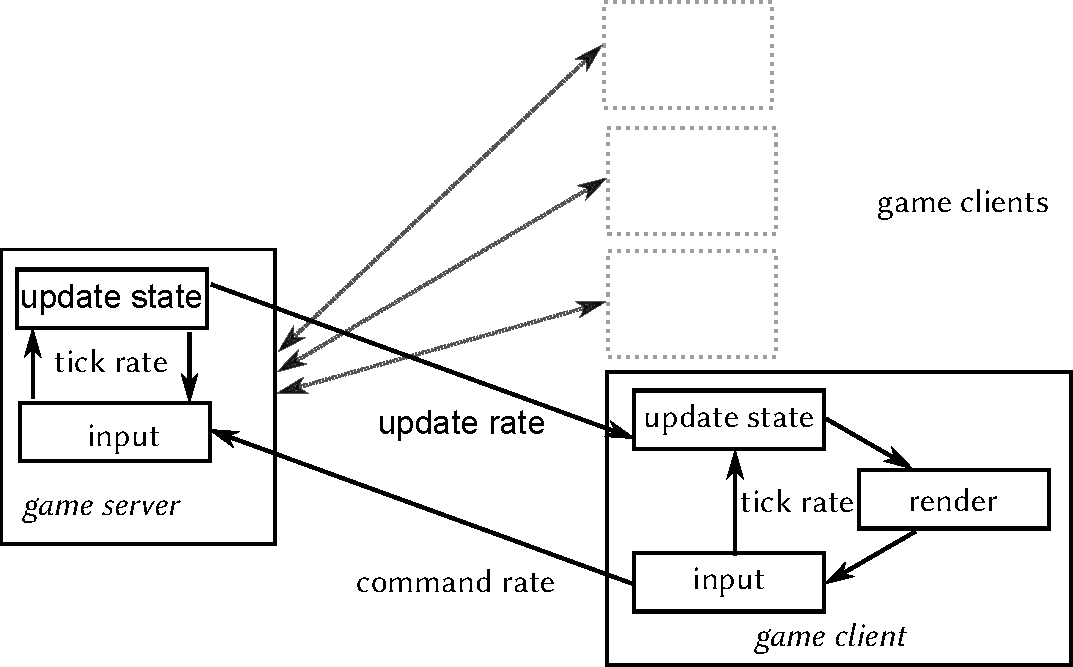
\includegraphics[width=1.0\columnwidth]{images/game-tick-rate.pdf}
% 		\caption{In typical online games.}
% 		\label{fig:tickrate-online}
% 	\end{subfigure}%
% 	~
% 	\begin{subfigure}[b]{0.5\textwidth}
% 
%		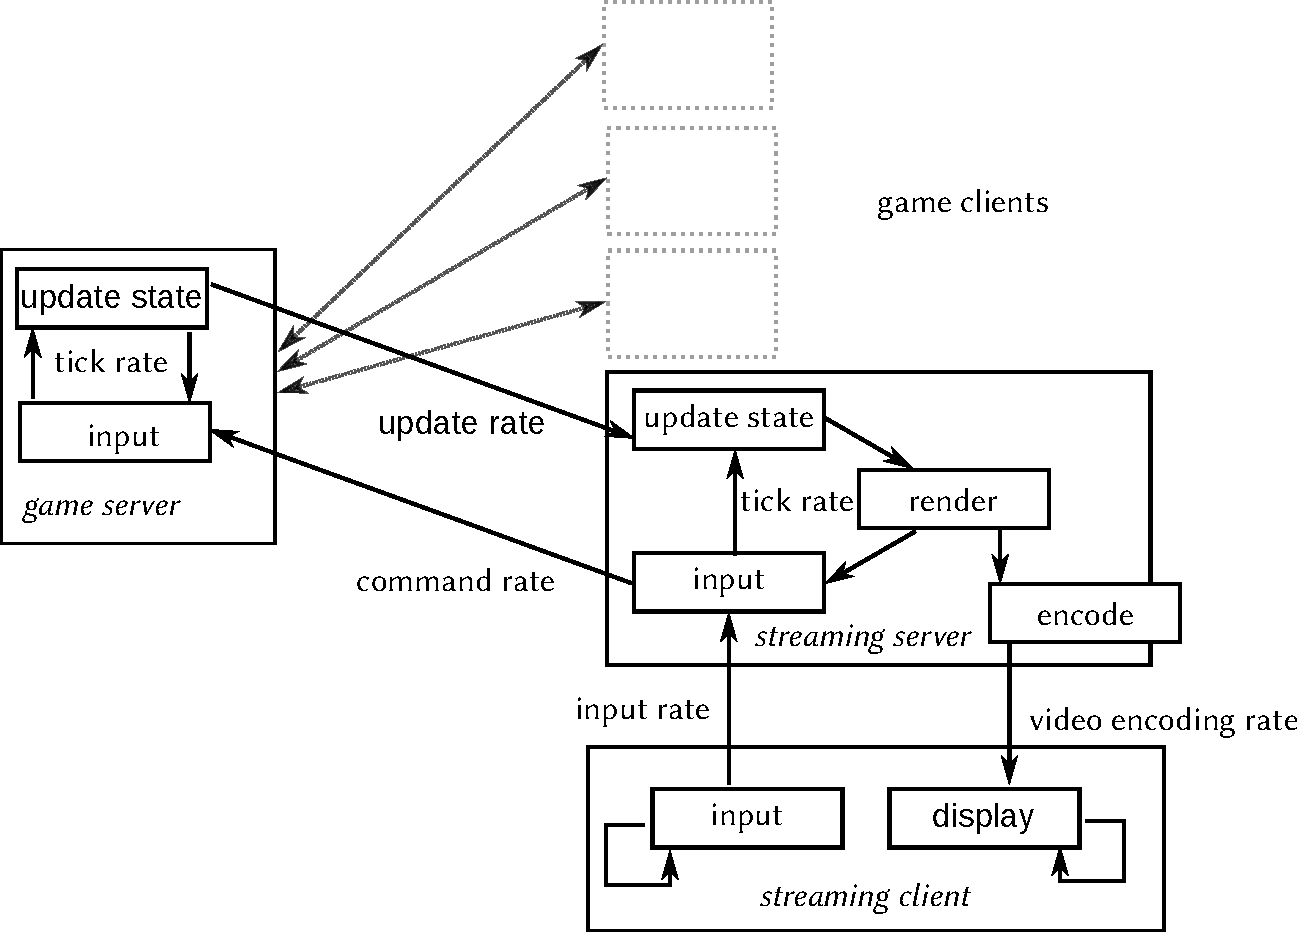
\includegraphics[width=1.0\columnwidth]{images/game-tick-rate-streamed.pdf}
% 		\caption{In a cloud gaming scenario.}
% 		\label{fig:tickrate-streamed}
% 	\end{subfigure}
% 	\caption{Interaction of the game client and server.}
% 	\label{fig:tickrates}
% \end{figure*}



% \begin{figure}[!t]
% 	\centering
% 	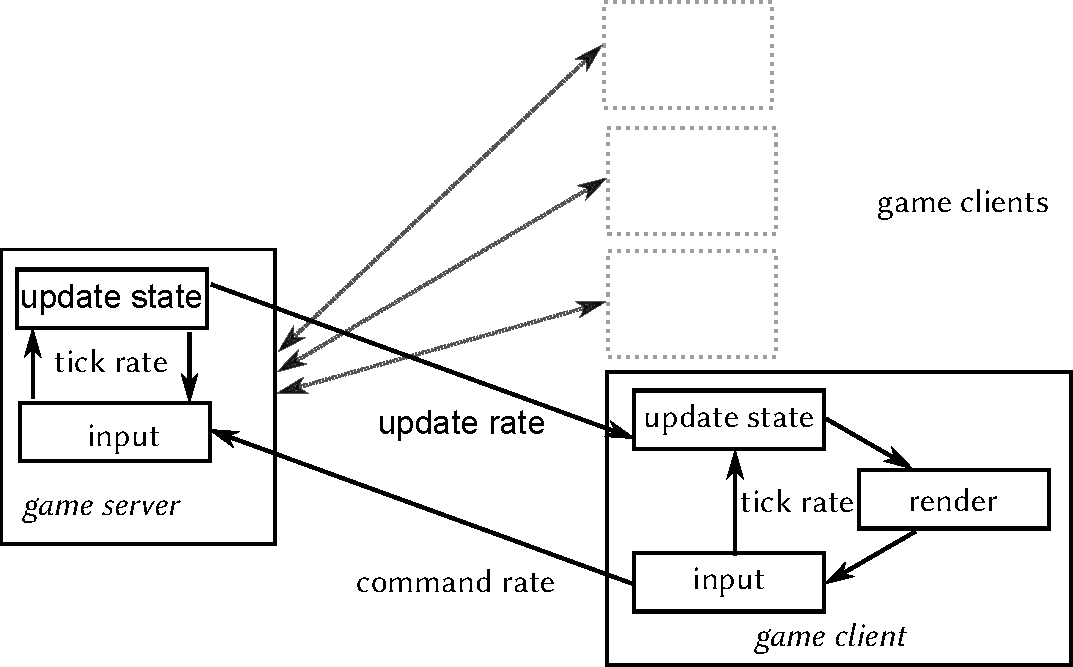
\includegraphics[width=1.0\columnwidth]{images/game-tick-rate.pdf}
% 	\caption{Interaction of client and server in typical online games.}
% \label{fig:tickrate-online}
% \end{figure}





% \begin{table}[!t]
% \caption{Exemplary table of some competitive and popular video game 
%tickrates that are either known, speculated upon, or derived by 
%counting update and command messages. Much of this information here is 
%guesswork from sometimes dubious sources and needs to be verified.}
% \label{tbl:tickrates}
% 	\centering
% 	\begin{tabu}{X[0.45]|X}
% 		\toprule
% 		\textbf{Video Game} & \textbf{Tickrate} \\
% 		\midrule
% 		CS: GO & Configurable \SI{64}{\hertz}/\SI{128}{\hertz} \\ \midrule
% 		Battlefield 4 & \SI{30}{\hertz} (\SI{10}{\hertz} for state outside 
%of close proximity to player). \SI{60}{\hertz}/\SI{120}{\hertz} 
%implemented on test servers. \\ \midrule
% 		Minecraft & max. \SI{20}{\hertz} \\ \midrule
% 		League of Legends & \SI{30}{\hertz} (guessed) \\ \midrule
% 		Dota 2 & \SI{30}{\hertz} \\ \midrule
% 		StarCraft II & supposedly either \SI{16}{\hertz} or \SI{32}{\hertz} 
%\\ \midrule
% 		Eve Online & \SI{1}{\hertz} \\ \midrule
% %		Sports Game 1 & \\ \midrule
% 		Project Cars & \SI{600}{\hertz} (Physics) \SI{250}{\hertz} (Input) 
%\\ %https://twitter.com/projectcarsgame/status/551340759858040833
% 		\bottomrule
% 	\end{tabu}
% \end{table}



% \subsection{Determining Video Game Popularity and Engagement}
% FUTURE WORK!

% Using Steam data as a popularity measure and get a grasp of which 
%games could be worthwhile to look at. Ties in to user engagement 
%metrics to determine the quality a game delivers in a current 
%situation. Alternative view: the more engaged players are to a game, 
%the more important is delivering a good quality (e.g. for streaming).

% For example, there might be a correlation between a game's price and 
%the average time it's been played, as 
%Figure~\ref{fig:tickrate-streamed}.


% Other  k-means clustering of steam/price data or other graphs

% \begin{figure}[!t]
% 	\centering
% 
%	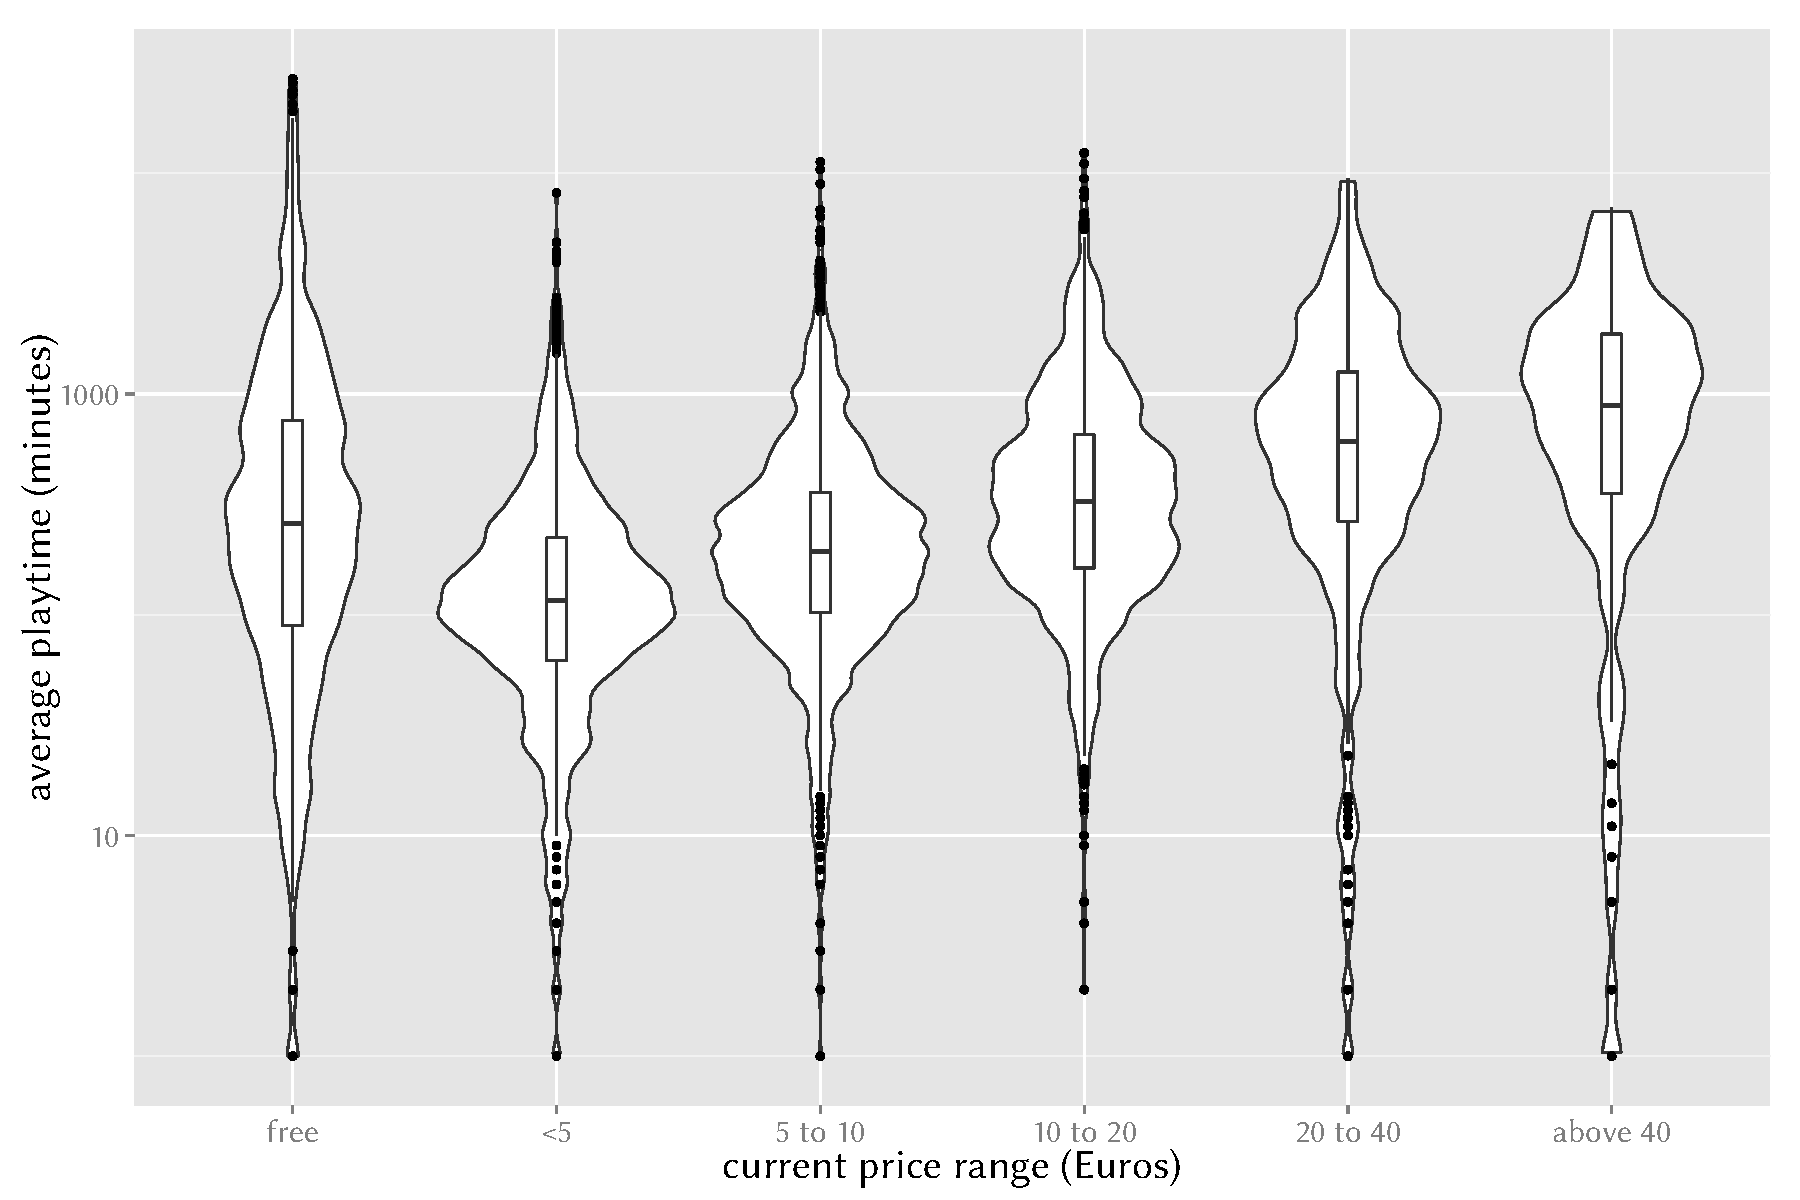
\includegraphics[width=1.0\columnwidth]{images/dampfviolinen-playtime.pdf}
% 	\caption{Game cost as a possible categorization and engagement 
%factor. Displayed is a violin plot of the current costs in relation to 
%the average playtime of individual games.s}
% \label{fig:cost-playtime-violin}
% \end{figure}

% Categorization dimensions viable for measuring online video game 
%quality:



%\footnote{\url{http://accidentalscientist.com/2014/12/why-movies-look-weird-at-48fps-and-games-are-better-at-60fps-and-the-uncanny-valley.html}}
%\url{https://stackoverflow.com/questions/17411/how-do-you-separate-game-logic-from-display}
%\url{http://higherorderfun.com/blog/2010/08/17/understanding-the-game-main-loop/}
